\documentclass{beamer}
\usetheme{metropolis}
\usepackage{graphicx}
\usepackage{amsmath}
\usepackage{tcolorbox}

\def\rcurs{{\mbox{$\resizebox{.16in}{.08in}{
\includegraphics{ScriptR}}$}}}
\def\brcurs{{\mbox{$\resizebox{.16in}{.08in}{
\includegraphics{BoldR}}$}}}
\def\hrcurs{{\mbox{$\hat \brcurs$}}}

\title{Electromagnetc Theory: PHYS330}
\author{Jordan Hanson}
\institute{Whittier College Department of Physics and Astronomy}

\begin{document}
\maketitle

\section{Summary}

\begin{frame}{Week 3 Summary}
\begin{enumerate}
\item Laplace's Equation
\begin{itemize}
\item One-dimension
\item Two-dimensions, three dimensions, uniqueness, boundaries
\end{itemize}
\item Separation of Variables: Boundary-value problems
\begin{itemize}
\item Cartesian coordinates
\item Spherical coordinates
\end{itemize}
\item Multipole Expansions
\begin{itemize}
\item Far-fields
\item Monopole and dipole terms
\item Electric Field of a Dipole
\end{itemize}
\end{enumerate}
\end{frame}

\section{Laplace's Equation: One Dimension}

\begin{frame}{Laplace's Equation: One dimension}
\alert{\textbf{Laplace's Equation in one dimension:}}
\begin{equation}
\frac{d^2V}{dx^2} = 0
\end{equation}
What is the solution?
\begin{equation}
V(x) = mx + b
\end{equation}
What is the magnitude of the E-field?
\begin{itemize}
\item A: $V(x)$
\item B: $x$
\item C: $b$
\item D: $m$
\end{itemize}
\end{frame}

\begin{frame}{Laplace's Equation: One dimension}
\begin{figure}
\centering
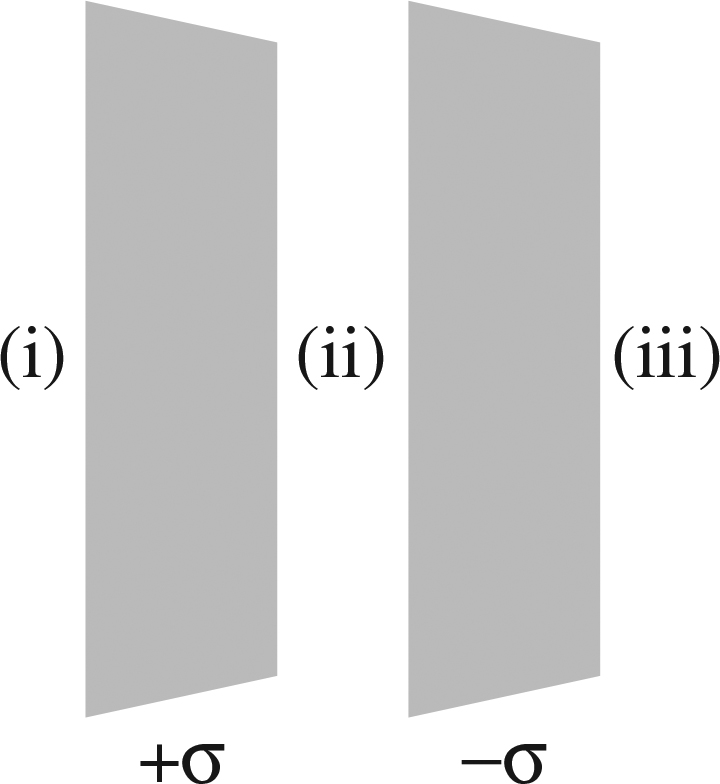
\includegraphics[width=6cm]{figures/2_23.jpg}
\caption{\label{fig:cap} The setup of a parallel plate capacitor.}
\end{figure}
\end{frame}

\begin{frame}{Laplace's Equation: One dimension}
\small
Suppose the negative side of the parallel plate capacitor is grounded, and the positive side is at a potential $V_0$.  Let the separation between the plates be $x_0$.  Further, let the positive plate occupy the yz plane, passing through the origin.  Find the E-field magnitude and direction by solving Laplace's equation. \\ \vspace{6cm}
\end{frame}

\begin{frame}{Laplace's Equation: One dimension}
\small
Show that the potential of a point charge at the origin satisfies Laplace's Equation for $r\neq 0$.  \textit{Use the form of the Laplacian in spherical coordinates.}\\ \vspace{6cm}
\end{frame}

\section{Boundary Conditions}

\begin{frame}{Boundary Conditions}
Let $V(x) = m x + b$.  If $V(-a) = V_0$, and $V(a) = -V_0$, what are valid expressions for $m$ and $b$?
\begin{itemize}
\item A: $b = 0$, and $m = -2V_0$
\item B: $b = a$, and $m = V_0/a$
\item C: $b = 0$, and $m = -V_0/a$
\item D: $b = V_0$, and $m = -V_0/a$
\end{itemize}
\end{frame}

\begin{frame}{Boundary Conditions}
Let $V(x) = m x + b$.  If $V(-a) = V_0$, and $V(a) = -V_0$, what is the electric field?
\begin{itemize}
\item A: $\frac{V_0}{a} \hat{x}$
\item B: $-\frac{V_0}{a} \hat{x}$
\item C: $V_0 \hat{x}$
\item D: $-V_0 \hat{x}$
\end{itemize}
\end{frame}

\begin{frame}{Boundary Conditions}
Suppose a potential function $V(x,y) \propto \left(A\exp(-kx) + B\exp(kx)\right)$.  Which of the following is true, if $V \to 0$ as $x \to \infty$?
\begin{itemize}
\item A: $A$ is 0
\item B: $A$ is 0
\item C: $A$ and $B$ are 0
\item D: Neither $A$ nor $B$ is 0
\end{itemize}
\end{frame}

\begin{frame}{Boundary Conditions}
Suppose a potential function $V(x,y) \propto \left(A\sin(kx) + B\cos(kx)\right)$.  Which of the following is true, if $V = 0$ as $x = 0$, and $V = 0$ as $x = a$?
\begin{itemize}
\item A: $B$ is 0, and $k = n\pi$
\item B: $A$ is 0, and $k = n\pi/(2a)$
\item C: $A$ and $B$ are 0
\item D: $B$ is 0, and $k = n\pi/a$
\end{itemize}
\end{frame}

\begin{frame}{Boundary Conditions}
\begin{columns}[T]
\begin{column}{0.5\textwidth}
Hyperbolic trigonometric functions:
\begin{itemize}
\item $\sinh(x) = \frac{1}{2}\left( e^{x} - e^{-x} \right)$
\item $\cosh(x) = \frac{1}{2}\left( e^{x} + e^{-x} \right)$
\item $\tanh(x) = \frac{\sinh(x)}{\cosh(x)}$
\end{itemize} \vspace{0.5cm}
Which of the following is zero?
\begin{itemize}
\item A: $\sinh(0)$
\item B: $\cosh(0)$
\item C: $\tanh(0)$
\item D: None
\end{itemize}
\end{column}
\begin{column}{0.5\textwidth}
Which of the following is one?
\begin{itemize}
\item A: $\sinh(0)$
\item B: $\cosh(0)$
\item C: $\tanh(0)$
\item D: None
\end{itemize}
Hyperbolic trigonometric functions are solutions to which equation?
\begin{itemize}
\item A: $\frac{df}{dx} = k$
\item B: $\frac{d^2f}{dx^2} = kx$
\item C: $\frac{d^2f}{dx^2} = k^2f$
\item D: $\frac{d^2f}{dx^2} = 0$
\end{itemize}
\end{column}
\end{columns}
\end{frame}

\begin{frame}{Boundary Conditions}
\alert{\textbf{Fourier's Trick}}: Imagine a vector with $n$ components:
\begin{equation}
\vec{v} = \sum_{i = 1}^n c_n \hat{x}_i
\end{equation}
In words, how do you solve for some $c_m$?
\begin{itemize}
\item A: Divide by $\hat{x}_i$
\item B: Take the dot product of both sides with $\hat{x}_{m}$
\item C: Take the dot product $\vec{v}$ and $\vec{u}$, and the sum the series
\item D: Integrate both sides with respect to $x$
\end{itemize}
\end{frame}

\begin{frame}{Boundary Conditions}
\alert{\textbf{Fourier's Trick}}: Imagine a vector with $n$ components:
\begin{equation}
\vec{v} = \sum_{i = 1}^n c_n \hat{x}_i
\end{equation}
In words, how do you solve for some $c_m$? Note that:
\begin{equation}
\vec{v} \cdot \hat{x}_m = \sum_{i = 1}^n c_n \hat{x}_i \cdot \hat{x}_m = c_m
\end{equation}
Why?  Because
\begin{align}
\hat{x}_i \cdot \hat{x}_j &= 0 \\
\hat{x}_i \cdot \hat{x}_i &= 1
\end{align}
\end{frame}

\begin{frame}{Boundary Conditions}
\alert{\textbf{Fourier's Trick}}: Imagine a known function that happens to be equal to a sum:
\begin{equation}
f(x) = \sum_{i = 1}^{\infty} c_n g_n(x)
\end{equation}
In words, how do you solve for some $c_m$?
\begin{itemize}
\item A: Multiply both sides by $g_m(x)$
\item B: Multiply both sides by $g_m(x)$ and integrate both sides with respect to $x$
\item C: Sum the infinite series and solve for $c_m$ with algebra
\item D: Integrate both sides with respect to $x$
\end{itemize}
\end{frame}

\begin{frame}{Boundary Conditions}
If it's true that a function can be written as an infinite series of functions with coefficients:
\begin{equation}
f(x) = \sum_{i = 1}^{\infty} c_n g_n(x)
\end{equation}
Then the functions $g_n(x)$ are said to be \textbf{\alert{complete}}, or a complete basis (just like vectors are a sum of basis vectors. Examples of complete sets of functions:
\begin{itemize}
\item sines and cosines (Fourier series) with the right frequencies
\item exponentials with the right rates multiplying $x$
\item Hyperbolic trigonometric functions (follows from exponentials)
\item Taylor series (polynomials with special coefficients: derivatives).
\end{itemize}
\end{frame}

\begin{frame}{Boundary Conditions}
The functions $g_n(x)$ are said to be \textbf{\alert{orthogonal}} if
\begin{equation}
\int_0^a f_n(y) f_m(y) dy = \delta_{n,m}0
\end{equation}
One example:
\begin{equation}
I_{n,m} = \int_L^{-L} \frac{\sin(n\pi x/L)}{\sqrt{L}}\frac{\sin(m\pi x/L)}{\sqrt{L}} dx
\end{equation}
What is the result of this integral?  How would you approach solving this?
\end{frame}

\begin{frame}{Boundary Conditions}
The \alert{\textbf{Fourier series}} representation of a function $f(x)$ is written:
\begin{equation}
S(x) = \frac{A_0}{2}+\sum_{i=1}^{\infty} \left( A_n \cos(nx) + B_n \sin(nx) \right)
\end{equation}
with
\begin{align}
A_n &= \frac{1}{\pi} \int_0^{2\pi} f(x) \cos(nx) dx \\
B_n &= \frac{1}{\pi} \int_0^{2\pi} f(x) \sin(nx) dx
\end{align}
\end{frame}

\begin{frame}{Boundary Conditions}
Let's obtain the \alert{\textbf{Fourier series}} coefficients $A_n$ and $B_n$ for a square-wave signal:
\begin{equation}
f(x) = 1, ~~ 0 \leq x \leq \pi, ~~ 0,  \pi < x \leq 2\pi 
\end{equation}
(Observe on board).  The result: $A_0 = 1.0$, all other $A_n = 0$, odd $B_n$ values follow $2/(n\pi)$, even $B_n = 0$ as well.
\end{frame}

\section{Separation of Variables}

\begin{frame}{Separation of Variables}
Laplaces' Equation:
\begin{equation}
\frac{\partial^2 V}{\partial x^2} + \frac{\partial^2 V}{\partial y^2} + \frac{\partial^2 V}{\partial z^2} = 0
\end{equation}
Assume the solution follows
\begin{equation}
V(x,y,z) = X(x) Y(y) Z(z)
\end{equation}
The Laplace equation then breaks into three separate ordinary differential equations. Application of boundary conditions to solve them (Asynchronous video content on Moodle).
\end{frame}

\begin{frame}{Separation of Variables}
\small
Laplaces' Equation in spherical coordinates:
\begin{equation}
\frac{1}{r^2}\frac{\partial}{\partial r} \left( r^2 \frac{\partial V}{\partial r}\right) + \frac{1}{r^2\sin\theta}\frac{\partial}{\partial \theta} \left( \sin\theta \frac{\partial V}{\partial \theta}\right) + \frac{1}{r^2\sin\theta}\left(\frac{\partial^2 V}{\partial \phi^2}\right) = 0 \label{eq:lap}
\end{equation}
Assuming \textit{azimuthal symmetry} means $V(r,\theta,\phi) = V(r,\theta)$ and $\partial V/ \partial \phi = 0$.  Thus, Eq. \ref{eq:lap} reduces and admits general solutions:
\begin{equation}
\frac{1}{r^2}\frac{\partial}{\partial r} \left( r^2 \frac{\partial V}{\partial r}\right) + \frac{1}{r^2\sin\theta}\frac{\partial}{\partial \theta} \left( \sin\theta \frac{\partial V}{\partial \theta}\right) = 0 \label{eq:lap2}
\end{equation}
Let the general solutions be separable:
\begin{equation}
V(r,\theta) = R(r) \Theta (\theta)
\end{equation}
\end{frame}

\begin{frame}{Separation of Variables}
The radial equation is
\begin{equation}
\frac{1}{R} \frac{d}{dr}\left(r^2 \frac{dR}{dr} \right) = l(l+1)
\end{equation}
Exercise: show that the solution is 
\begin{equation}
R(r) = A r^l + B r^{-(l+1)}
\end{equation}
(The derivative operator distributes over addition, so the two solutions can be checked separately, or together). \\ \vspace{0.5cm}
\textbf{What are the units of $R(r)$?  What are the units of $A$ and $B$?}
\end{frame}

\begin{frame}{Separation of Variables}
The radial equation is
\begin{equation}
\frac{1}{R} \frac{d}{dr}\left(r^2 \frac{dR}{dr} \right) = l(l+1)R(r)
\end{equation}
Exercise: show that the solution is 
\begin{equation}
R(r) = A r^l + B r^{-(l+1)}
\end{equation}
(The derivative operator distributes over addition, so the two solutions can be checked separately, or together). \\ \vspace{0.5cm}
\textbf{What are the units of $R(r)$?  What are the units of $A$ and $B$?}
\end{frame}

\begin{frame}{Separation of Variables}
The polar equation is
\begin{equation}
\frac{d}{d\theta}\left(\sin\theta \frac{d\Theta}{d\theta} \right) = -l(l+1)\sin\theta \Theta(\theta)
\end{equation}
The solutions are \alert{complete}, and \alert{orthogonal}, and known as Legendre polynomials:
\begin{equation}
\Theta(\theta) = P_l(\cos\theta)
\end{equation}
Defined by the \textit{Rodrigues formula}:
\begin{equation}
P_l(x) = \frac{1}{2^ll!} \left(\frac{d}{dx}\right)^l (x^2 -1)^l
\end{equation}
\end{frame}

\begin{frame}{Separation of Variables}
Exercise: show that 
\begin{equation}
P_3(x) = (5x^3 - 3x)/2
\end{equation}
\alert{\textbf{What is the result of the following integrals?}}
\begin{align}
I_1 &= \int_{-1}^{1} P_2(x) P_3(x) dx \\
I_2 &= \int_{-1}^{1} P_3(x) P_3(x) dx
\end{align}
If the integer $l$ is \textit{even/odd}, the $l$-th order Legendre polynomial will be
\begin{itemize}
\item A: odd/even
\item B: odd/odd
\item C: even/even
\item D: even/odd
\end{itemize}
\end{frame}

\begin{frame}{Separation of Variables}
The general solution is a sum of individual solutions:
\begin{equation}
V(r,\theta) = \sum_{i = 0}^{\infty} \left( Ar^l + B/r^{l+1} \right) P_l(\cos\theta)
\end{equation}
The coefficients may be found via Fourier's Trick.
\end{frame}

\begin{frame}{Example 3.9: Professor on Board}
A specified charge density $\sigma_0(\theta)$ is glued over the surface of a spherical shell of radius $R$.  Find the resulting potential inside and outside the sphere. \\
\begin{enumerate}
\item Inside the sphere, $B = 0$ to avoid a singularity at the origin (center of sphere).
\item Outside the sphere, $A = 0$ to ensure $V \to 0$ as $r \to \infty$.
\item General boundary conditions at $r = R$: potential is continuous ($-\int \vec{E} \cdot d\vec{l} = 0$).
\item Coefficients of same order $l$ have a relationship.
\item E-field has a discontinuity at the boundary.
\item Fourier's trick to get the coefficients, after specifying $\sigma_0(\theta)$.
\end{enumerate}
\end{frame}

\section{Multipole Expansion}

\begin{frame}{Multipole Expansion}
Imagine a \textit{physical dipole} with $q$ at $\hat{r}' = d/2 hat{z}$ and $-q$ at $\hat{r}' = -d/2 \hat{z}$.  Show that (professor example) 
\begin{equation}
V(r,\theta) = \frac{kqd}{r^2} P_1(\cos\theta)
\end{equation}
\begin{enumerate}
\item Far-field on script-r's
\item Subtract
\item Simplify
\item Note that $P_1(x) = x$.
\end{enumerate}
\end{frame}

\begin{frame}{Multipole Expansion}
Can't you break \textit{any} charge distribution into a collection of monopoles, dipoles, quadrupoles, ... ? We will show next time that
\begin{equation}
\boxed{
\frac{1}{\rcurs} = \frac{1}{r} \sum_{n=0}^{\infty} \left( \frac{r'}{r} \right)^n P_n(\cos\theta)
}
\end{equation}
\end{frame}

\section{Conclusion}

\begin{frame}{Week 3 Summary}
\begin{enumerate}
\item Laplace's Equation
\begin{itemize}
\item One-dimension
\item Two-dimensions, three dimensions, uniqueness, boundaries
\end{itemize}
\item Separation of Variables: Boundary-value problems
\begin{itemize}
\item Cartesian coordinates
\item Spherical coordinates
\end{itemize}
\item Multipole Expansions
\begin{itemize}
\item Far-fields
\item Monopole and dipole terms
\item Electric Field of a Dipole
\end{itemize}
\end{enumerate}
\end{frame}

\end{document}
